\section{Robot Hand Design and Intelligent Mechanisms}
\label{sec:hands}

The mechanical platform determines what a tactile sensing system can achieve. This section reviews the design spectrum from parallel grippers to multi-fingered hands, the open-source revolution that democratized dexterous manipulation research, actuation methods, and three classes of intelligent mechanisms that embed physical intelligence into the gripper structure.

\subsection{Design Spectrum: Grippers to Dexterous Hands}

Robot end-effectors span a continuum from simple parallel grippers (2 fingers, 1 DoF) to fully anthropomorphic hands (5 fingers, 20+ DoF). Parallel grippers dominate industrial deployment due to their simplicity and reliability, but suffer from poor shape adaptation, inability to maintain continuous contact, and vulnerability with thin or multiple objects. Dexterous hands offer diverse grasp types and in-hand manipulation but introduce control complexity, combinatorial explosion of contact states, high cost, and frequent hardware failures~\cite{bicchi2000simplicity,bicchi2000grasping}.

Bicchi's landmark argument for simplicity~\cite{bicchi2000simplicity} resolved this tension by introducing \emph{underactuation} (fewer actuators than joints) and \emph{synergy} (coordinated multi-joint patterns), demonstrating that most everyday grasps can be explained by 2--3 principal synergies extracted via PCA. This insight directly shaped modern affordable hands including the SoftHand family and LEAP Hand.

\begin{figure}[t]
\centering
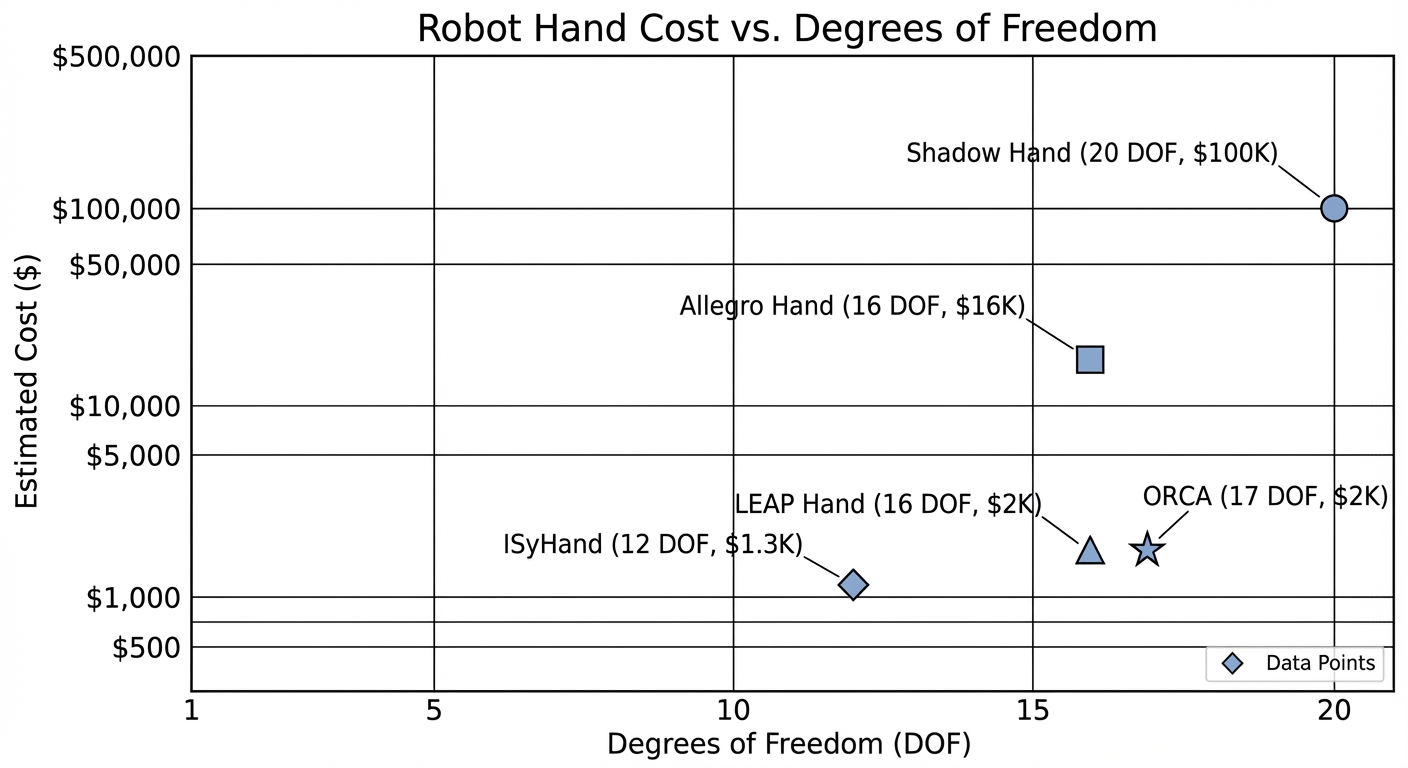
\includegraphics[width=\columnwidth]{../assets/figures/ch04/fig_4_2_hand_cost_performance_academic.png}
\caption{Cost--performance landscape of dexterous robot hands. The open-source revolution (2023--2025) reduced entry costs by 50$\times$, from Shadow Hand (\$100K+) to LEAP Hand (\$2K) and ISyHand (\$1.3K), while maintaining or improving manipulation performance.}
\label{fig:hand_cost_performance}
\end{figure}

\subsection{The Open-Source Revolution}

Since 2023, low-cost open-source dexterous hands have fundamentally transformed the research ecosystem by reducing the entry cost by 50$\times$. Table~\ref{tab:hands} compares the major platforms.

\begin{table*}[t]
\caption{Comparison of Dexterous Robot Hands}
\label{tab:hands}
\centering
\begin{tabular}{@{}lcccccc@{}}
\toprule
\textbf{Hand} & \textbf{Cost} & \textbf{DoF} & \textbf{Actuation} & \textbf{Tactile} & \textbf{Open-Source} & \textbf{Year} \\
\midrule
Shadow Hand & \$100K+ & 24 & Tendon/pneumatic & BioTac (opt.) & No & 1990s \\
Allegro Hand & \$16K & 16 & Direct drive & No & No & 2012 \\
LEAP Hand~\cite{shaw2023leap} & \$2K & 16 & Direct drive & No & Yes & 2023 \\
ISyHand~\cite{richardson2025isyhand} & \$1.3K & var. & Direct drive & No & Yes & 2025 \\
ORCA~\cite{christoph2025orca} & \$2K & 17 & Tendon & Yes & Yes & 2025 \\
F-TAC Hand~\cite{zhao2025ftac} & --- & var. & var. & 17 sensors & Partial & 2025 \\
\bottomrule
\end{tabular}
\end{table*}

\textbf{LEAP Hand}~\cite{shaw2023leap} (CMU, RSS 2023, 200+ citations) established the open-source paradigm: a 3D-printable, 4-finger, 16-DoF hand costing \$2K that outperforms the \$16K Allegro Hand on benchmark tasks. Its novel kinematic structure reproduces the essential degrees of freedom of the human hand using only low-cost servo motors and 3D-printed components. The design philosophy---``maximum dexterity at minimum cost''---catalyzed a wave of follow-on work.

\textbf{ISyHand}~\cite{richardson2025isyhand} (MPI, IEEE Humanoids 2025) further reduced cost to \$1.3K while introducing an \emph{articulated palm} that increases overall dexterity with modest sacrifice in anthropomorphism. Assembly requires only 4 hours from off-the-shelf Dynamixel motors and 3D-printed parts.

\textbf{ORCA}~\cite{christoph2025orca} (ETH Zurich) provides a 17-DoF tendon-driven hand with \emph{integrated tactile sensors}, built for under 2{,}000~CHF in 8 hours. Key reliability features---popping joints, auto-calibration, and tensioning systems---reduce maintenance complexity, enabling continuous learning without frequent hardware intervention. The commercial spinoff Mimic Robotics is pursuing factory-grade deployment.

The \textbf{F-TAC Hand}~\cite{zhao2025ftac} (\emph{Nature Machine Intelligence}, 2025) demonstrated the value of sensor-integrated co-design: 17 vision-based tactile sensors placed according to contact probability distributions cover 70\% of the hand surface at 0.1~mm resolution, achieving 100\% multi-object grasp success---a metric that no non-tactile hand has matched.

The Allegro Hand (\$16K, Wonik Robotics) served as the de facto research standard prior to the open-source wave and remains prominent in sim-to-real work including DeXtreme~\cite{handa2023dextreme} and the RGMC competition~\cite{yu2025rgmc}. Wonik's ongoing Digit Plexus integration with Meta FAIR represents a step toward standardized sensor-hand interfaces.

\subsection{Actuation Methods}

Four actuation methods dominate, each with distinct trade-offs:

\textbf{Direct drive} couples motors directly to joints (Allegro, LEAP). Advantages: fast control response, simple kinematics, precise position control. Disadvantage: motor size constrains finger miniaturization.

\textbf{Tendon-driven} designs place actuators remotely and transmit force via tendons (SoftHand~\cite{catalano2014softhand}, ORCA~\cite{christoph2025orca}, Shadow Hand). Advantages: finger miniaturization, natural compliance, reduced distal mass. Disadvantage: tendon routing complexity, friction losses, wear.

\textbf{Hydraulic} actuation (Sanctuary AI Phoenix Gen~8) achieves high power density with 20~DoF and 5~mN tactile sensitivity---the most advanced tactile integration among commercial humanoids. The 50$\times$ faster, 6$\times$ cheaper miniaturized valves represent a significant engineering achievement. Disadvantage: system complexity and cost.

\textbf{Pneumatic} actuation using McKibben muscles~\cite{alabeach2017vsa} provides inherent compliance and variable stiffness through antagonistic arrangements. Well suited for safe human-proximity operation but offers lower control precision than electric alternatives.

\subsection{Intelligent Mechanisms}
\label{sec:mechanisms}

Three classes of mechanisms embed ``physical intelligence'' into gripper design, reducing the burden on sensing and learning systems.

\subsubsection{Underactuation}

Underactuated hands use fewer actuators than joints, with remaining joints determined passively by springs or mechanical stops. The core value is \emph{automatic shape adaptation}: the mechanism itself, not a control algorithm, conforms to object geometry.

The Pisa/IIT SoftHand family exemplifies this approach. SoftHand~1~\cite{catalano2014softhand} (\emph{IJRR}, 2014, 500+ citations) drives 19 joints with a single actuator via adaptive synergy---all joints coordinate along the first principal synergy, and tendons slip on contact to automatically expand the contact area. SoftHand~2~\cite{dellasantina2018softhand2} (\emph{IEEE T-RO}, 2018) added a second actuator with friction-based actuation expansion for more diverse grasp types. Capsi-Morales et al.~\cite{capsimorales2020palm} extended adaptability to the palm itself by sectioning and connecting palm segments via underactuation.

\subsubsection{Variable Stiffness Actuators (VSA)}

VSAs enable a single mechanism to transition between compliant and stiff states, addressing the fundamental tension between compliance (needed for safe contact) and rigidity (needed for stable grasping). Four implementation approaches have been demonstrated: (1)~parallel beam with slider-adjustable effective length, achieving 70.9$\times$ stiffness ratio with ArUco marker-based vision force sensing~\cite{fu2023vsa}; (2)~McKibben muscle antagonistic arrangement enabling independent pose-stiffness control with 150\%+ stiffness increase~\cite{alabeach2017vsa}; (3)~SMA actuation combined with SMP stiffness switching, achieving 55$\times$ change per hinge~\cite{wang2017sma}; and (4)~particle jamming with fiber-reinforced pneumatic actuators for 10$\times$+ stiffness enhancement~\cite{wei2016jamming}.

\subsubsection{Active Surfaces}

Active surfaces drive the gripper's contact surface itself---typically via belts or rollers---enabling manipulation while maintaining contact. This addresses thin-object approach (pulling cards from a table), in-grasp repositioning (adjusting object position without releasing), and continuous-contact manipulation~\cite{kim2024lbh,wang2025belt}. The key insight is that \emph{continuous contact is easier to control and more stable than discrete release-and-regrasp}, because it eliminates the uncertainty of contact state transitions.

\subsubsection{Temporal Integration}

The most powerful approach combines all three mechanisms in temporal sequence: (1)~underactuation for initial shape adaptation during approach, (2)~VSA for stiffness transition to lock the grasp, and (3)~active surfaces for in-grasp manipulation and repositioning. This sequence mirrors the natural human grasping flow---approach, grasp, adjust---through purely mechanical means. The synergy of these three mechanisms creates capabilities beyond the sum of their individual contributions, particularly for factory automation scenarios involving thin objects, multiple objects, and precision repositioning. This physical intelligence concept forms one axis of the mechanism--tactile--learning triangle proposed in Section~\ref{sec:discussion}.
